\documentclass[]{style}
\usepackage{amsmath,amssymb}
\usepackage{graphicx}
\usepackage{booktabs}
\usepackage{array}
\usepackage{tabularx}
\usepackage{enumitem}
\graphicspath{{textcards/}{bench/}}
\usepackage{xcolor}
\newcommand{\cardbox}[3]{%
  \fcolorbox{black!35}{black!3}{\begin{minipage}[t][4.95cm][t]{0.305\textwidth}\footnotesize\raggedright
  \textbf{#1}\hfill{\color{black!55}#2}\par\vspace{2pt}\hrule\vspace{3pt}
  {\scriptsize #3}\end{minipage}}}

\title{\fontsize{0.6cm}{0.72cm}\selectfont Encoding Cellular Perturbation\\[0.3cm] with Large Language Models}

% \author{Dennis~Wu}
% \author{Ali~ElSheikh}
% \author{Payam~Dibaeinia}
% \author{Sudarshan~Babu}
% \author{Jason~Perera}
% \author{Aly~A~Khan}
% \author{Han~Liu}

\abstract{
In this work, we explore the possibilities to encode cellular perturbation using large language models (LLMs).
Most virtual cell models represent each perturbation with a learned embedding, so they can only model perturbations seen
during training.
Therefore, we propose to use LLMs to encode each perturbation through its description.
We collect 10,801 descriptions of different perturbations from NCBI Gene, the Gene Ontology, PubChem and curated drug and
cytokine tables. They cover CRISPRa, CRISPRi and knockout genes, drugs and cytokines.
Next, we use the Qwen3 embedding model to turn each description into a vector.
We test the Qwen3 embeddings with a pool of simple baseline models on six perturbation prediction datasets from Virtual
Cell Bench, using the benchmark's own folds.
Surprisingly, models using the Qwen3 embeddings improve almost uniformly compared to the same models without them.
When the test perturbations are new, the model with the Qwen3 embedding wins in 93 of 105 pairs, with a median gain of
0.4 to 0.9 on the ability scale.
}

\begin{document}
\maketitle

% ---------------------------------------------------------------------------
\section{Introduction}

Virtual Cell Bench \citep{companion} scores perturbation models on items. An item is one perturbation in one cell
context, such as one drug in one cell line at one dose. Every model gives a predicted change in gene expression for every
item. The benchmark turns these predictions into a pass or fail and fits an item response model, which gives each model
an ability and each item a difficulty on one shared scale.

Each model also needs a feature that says which perturbation it is. The benchmark uses a fixed feature per screen. For
genetic screens it is a gene embedding built from control cells. For Tahoe-100M it is a Morgan fingerprint of the drug.
For sciPlex3 and the two cytokine screens it is a one-hot label. A one-hot label carries no information about a
perturbation that was never seen in training, and the other two carry only a little.

A text card is a short written description of the perturbation, taken from curated databases. Every gene, drug and
cytokine has one, whether or not it was measured. This report explains how we build, embed and test the cards.

% ---------------------------------------------------------------------------
\section{Building the Cards}

Every perturbation gets one card. The card says what the perturbation is. It never says how cells responded in our data,
so the test responses cannot leak into it. Each card starts with fixed fields and then adds a free-text description.

\begin{itemize}[leftmargin=*,itemsep=1pt,topsep=2pt]
\item \textbf{Genes} (CRISPRi, CRISPRa and knockout). Fields: the gene name and how it was perturbed. Text: the NCBI
Gene summary and the Gene Ontology biological process terms, fetched from mygene.info \citep{mygene}. We look up the
exact gene symbol first and use an alias only when the symbol is not found and the alias matches exactly.
\item \textbf{Drugs}. Fields: targets, mechanism of action and approval status from the Tahoe drug table \citep{tahoe},
or target and pathway labels from sciPlex3 \citep{srivatsan2020}. Text: the PubChem compound description
\citep{pubchem}.
\item \textbf{Cytokines}. Fields: the genes that encode the cytokine, its receptor genes and its family, from a table we
curated by hand. Text: the NCBI Gene summaries of the ligand and receptor genes.
\end{itemize}


\begin{figure}[t]
\centering
\cardbox{Gene (CRISPRi): CDK9}{190 words}{\textbf{Perturbation:} CDK9. \textbf{Type:} CRISPR interference knockdown (gene expression reduced). \textbf{Target gene:} CDK9. CDK9 (cyclin dependent kinase 9). The protein encoded by this gene is a member of the cyclin-dependent protein kinase (CDK) family. CDK family members are highly similar to the gene products of S. cerevisiae cdc28, and S. pombe cdc2, and known as important cell cycle regulators. This kinase [\dots]}
\hfill
\cardbox{Drug: Trametinib}{120 words}{\textbf{Perturbation:} Trametinib. \textbf{Type:} small-molecule compound. \textbf{Targets:} MAP2K1, MAP2K2. \textbf{Mechanism of action:} MEK inhibitor (inhibitor/antagonist). \textbf{Approved for human use:} yes. \textbf{ChEMBL ID:} CHEMBL2103875. Trametinib is a pyridopyrimidine that is used (as its dimethyl sulfoxide addition compound) for the treatment of patients with unresectable or metastatic melanoma with BRAF V600E or V600K mutations, and who have not received prior BRAF inhibitor treatment. [\dots]}
\hfill
\cardbox{Cytokine: IFN-gamma}{343 words}{\textbf{Perturbation:} IFN-gamma. \textbf{Type:} recombinant cytokine (extracellular signalling protein). \textbf{Cytokine family:} type II interferon. \textbf{Encoded by:} IFNG. \textbf{Receptor genes:} IFNGR1, IFNGR2. IFNG (interferon gamma). This gene encodes a soluble cytokine that is a member of the type II interferon class. The encoded protein is secreted by cells of both the innate and adaptive immune systems. The active protein is a homodimer [\dots]}

\caption{One example card for each kind of perturbation, cut to the first 60 words (the full length is given at the top
right). Field names are in bold. The whole card, not only the free text, is given to the embedding model.}
\label{fig:cards}
\end{figure}

\Cref{fig:cards} shows one card of each kind. All cards also list which datasets measured the perturbation, how many cell contexts, and the doses. The cards cover
9,591 CRISPRi, 236 CRISPRa and 233 knockout genes, 565 drugs, 90 human cytokines for the Parse PBMC screen
\citep{parsepbmc}, and 86 mouse cytokines for the Immune Dictionary \citep{cui2024} (79 of them also in Parse). The
median card has 51 words for drugs, 107 to 186 words for genes, and 373 words for cytokines.

% ---------------------------------------------------------------------------
\section{From a Card to a Feature}

We embed each card with Qwen3-Embedding-4B \citep{qwen3emb}, a text embedding model with 4 billion parameters. The card
is embedded as a document, with no instruction in front of it. Each card becomes one vector of 2,560 numbers.

Within each screen we reduce the vectors to 32 numbers with principal component analysis. We fit this on the
perturbations of that screen only. The model's feature is these 32 numbers joined to a one-hot code for the cell
context, plus the log dose when the screen has more than one dose. This replaces the screen's built-in perturbation
feature. Nothing else in the model or the data changes.

% ---------------------------------------------------------------------------
\section{How We Test the Cards}

\paragraph{Screens and splits.} We use six screens: Norman \citep{norman2019} (CRISPRa, K562 cells), Replogle
\citep{replogle2022} (CRISPRi, K562 essential genes), sciPlex3 (drugs, three cell lines), Tahoe-100M (drugs, 50 cell
lines), Parse PBMC (cytokines, 12 donors and 18 cell types) and the Immune Dictionary (cytokines injected into mice,
13 lymph node cell types). The main test is the unseen-perturbation split: the benchmark holds out whole perturbations in
five folds, so every test perturbation is new to the model. We also run the unseen-combination split on the two cytokine
screens, where each test perturbation was seen in other cell types but not in the test cell type.

\paragraph{Models.} We take every model in the benchmark pool that reads a perturbation feature: k-nearest neighbours,
ridge regression, Gaussian processes, PCA regression, two multilayer perceptrons, and versions of these trained on 10\%
or 30\% of the training data. Each model is fitted twice on the same folds, once with the built-in feature and once with
the text card. Models with no perturbation feature, such as the mean shift, are not refitted.

\paragraph{Scoring.} A model passes an item when the Pearson correlation between its predicted and measured expression
shift, over the 2,000 most variable genes, is higher than the correlation of the mean shift. The mean shift is the
average response of the training perturbations in the same cell context. We place the text models on each screen's published scale with the
item difficulties held fixed, the same way the benchmark adds any new model. As a check, we also refitted every scale
with the text models included. The order of all models changed very little: the Spearman correlation between the two
orders was 0.994 or higher on every screen.

% ---------------------------------------------------------------------------
\section{Results}

\paragraph{New perturbations.} \Cref{tab:main} and \Cref{fig:pairs} compare each model with its own twin. The text card
wins in 93 of 105 pairs. The median gain is between 0.41 and 0.86 on every screen. The best model overall uses the text card on Norman, Replogle, Tahoe and
the Immune Dictionary. On sciPlex3 and Parse the best model still uses the built-in feature: PCA regression on
sciPlex3 ($-0.36$ against $-0.50$) and 20-nearest neighbours on Parse ($-0.20$ against $-1.31$).

\begin{table}[t]
\centering
\caption{Unseen perturbations. Pairs: models fitted with both features. Wins: pairs where the text card has the higher
ability. Gain: median of text ability minus built-in ability. The last two columns give the best ability reached with
each feature. Ability is on each screen's own scale.}
\label{tab:main}
\small
\begin{tabular}{llrrrrr}
\toprule
Screen & Built-in feature & Items & Wins & Gain & Best built-in & Best text \\
\midrule
Norman 2019 & gene embedding from control cells & 225 & 21/22 & $+0.51$ & $+2.74$ & $+3.18$ \\
Replogle 2022 & gene embedding from control cells & 1,660 & 21/22 & $+0.86$ & $+0.39$ & $+1.06$ \\
sciPlex3 & one-hot, context, dose & 2,092 & 6/9 & $+0.41$ & $-0.36$ & $-0.50$ \\
Tahoe-100M & Morgan fingerprint, context, dose & 39,698 & 12/15 & $+0.48$ & $-1.04$ & $-0.47$ \\
Parse PBMC & one-hot, context & 10,744 & 21/22 & $+0.67$ & $-0.20$ & $-1.31$ \\
Immune Dictionary & one-hot, context & 757 & 12/15 & $+0.50$ & $-1.10$ & $-0.85$ \\
\bottomrule
\end{tabular}
\end{table}

\begin{figure}[t]
\centering
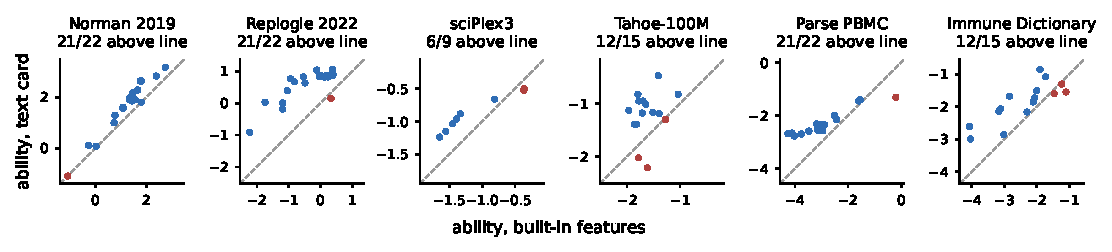
\includegraphics[width=\textwidth]{fig_pairs.pdf}
\caption{Each dot is one model fitted twice. The x axis is its ability with the built-in feature and the y axis is its
ability with the text card. Blue dots lie above the dashed line, where the text card is better; red dots lie below it.}
\label{fig:pairs}
\end{figure}

\paragraph{What the embedding holds.} We grouped the measured responses of each screen into clusters, using the half of
the perturbations with the strongest response. We then asked how often a perturbation's nearest neighbours by text fall
in its own response cluster. The rate was 2.9 times chance on Norman, 2.7 on Replogle and 2.2 on sciPlex3, but only 1.3
on Tahoe and 1.2 on Parse.

\paragraph{Cytokines.} The cards help on Parse, but the absolute abilities stay low. To see why, we compared several
ways of saying two cytokines are alike: text card similarity, a shared receptor gene, and the same family. All three
predicted response similarity equally weakly (Spearman 0.08 on Parse). Many cytokines give a weak response in most cell
types, and two cytokines of the same family respond only a little more alike than two random ones (correlation 0.20
against 0.12 on average).

\paragraph{New combinations.} On the unseen-combination split the test perturbation was already measured in other cell
types. We built ridge models that add a term for how a perturbation's response differs between cell types, with three
sources for that term: the measured responses, the text card, or both. The model with measured responses is the best
model on the Immune Dictionary ($+3.99$, against $+3.36$ for the best published model). Adding the text card to it does
not help ($+3.97$), and the text card alone does worse ($+2.99$). On Parse every one of these models stays below the best
published model.

% ---------------------------------------------------------------------------
\section{Text Cards in CPA}

To test a deep generative model, we put the cards into CPA \citep{cpa} (cpa-tools 0.8.8).
CPA learns a vector for each perturbation, adds it to a latent code of the control cell, and decodes the sum into gene
expression. We run CPA in two ways on the same folds:

\begin{itemize}[leftmargin=*,itemsep=1pt,topsep=2pt]
\item \textbf{Own embedding}: CPA learns its perturbation vectors from scratch. A perturbation held out in the test fold
never gets trained, so its vector stays at its random start.
\item \textbf{Text card}: we reduce the card vectors to 128 numbers with PCA, scale each to unit length, and load them
into CPA's perturbation table as fixed values. CPA still learns its own linear layer from these values into the latent
space. A new perturbation therefore gets a vector that reflects its description.
\end{itemize}

Both versions use the same settings: a 64-dimensional latent space, a negative binomial loss, up to 300 epochs with
early stopping, and up to 200 cells per training item plus all control cells. To predict an item, we pass control cells of the test context through CPA with the test perturbation and
again with no perturbation. The predicted shift is the difference of the two means, in log counts per 10,000 over the
2,000 most variable genes. These shifts are scored and placed on the published scales in the same way as above.

We run this on Norman, sciPlex3 and the Immune Dictionary with five folds each (\Cref{tab:cpa}).

\begin{table}[h]
\centering
\caption{CPA with its own perturbation embedding and with the text card. Runs in progress.}
\label{tab:cpa}
\small
\begin{tabular}{llrrr}
\toprule
Screen & Split & Own embedding & Text card & Best published \\
\midrule
Norman 2019 & unseen perturbation & -- & -- & $+2.74$ \\
sciPlex3 & unseen perturbation & -- & -- & $-0.36$ \\
sciPlex3 & unseen combination & -- & -- & $+0.06$ \\
Immune Dictionary & unseen perturbation & -- & -- & $-0.93$ \\
Immune Dictionary & unseen combination & -- & -- & $+3.36$ \\
\bottomrule
\end{tabular}
\end{table}

% ---------------------------------------------------------------------------
\section{Limits}

We used one embedding model. Every model was fitted once with one random seed; the error bars come from the item
response fit only. Some drug cards are short because little curated text exists for them.

{\small
\bibliographystyle{acl_natbib}
\bibliography{benchmark,textcards}
}

\end{document}
